% !TeX encoding = UTF-8
% !TeX spellcheck = pl_PL

% $Id:$
%% Konfiguracja:
\newcommand{\formakursu}{Projekt}
\newcommand{\kurs}{Teoria i metody optymalizacji}
\newcommand{\doctype}{Harmony Search}
\newcommand{\osobaA}{Artur \textsc{Gasi\'nski}, 218685}
\newcommand{\osobaB}{Bartosz \textsc{Lenartowicz}, 218518}
\newcommand{\termin}{wt 9:15-11:00}
%wpisz imię i nazwisko prowadzącego
\newcommand{\prowadzacy}{Dr in\.{z}. Ewa \textsc{\'Szlachcic}}
\documentclass[10pt, a4paper]{article}
\usepackage{listings}

\usepackage{indentfirst}
\usepackage{graphicx}
\usepackage{verbatim}
\usepackage[edges]{forest}
\usepackage{url}
\usepackage{hyperref}

\definecolor{foldercolor}{RGB}{124,166,198}
\tikzset{pics/folder/.style={code={%
			\node[inner sep=0pt, minimum size=#1](-foldericon){};
			\node[folder style, inner sep=0pt, minimum width=0.3*#1, minimum height=0.6*#1, above right, xshift=0.05*#1] at (-foldericon.west){};
			\node[folder style, inner sep=0pt, minimum size=#1] at (-foldericon.center){};}
	},
	pics/folder/.default={20pt},
	folder style/.style={draw=foldercolor!80!black,top color=foldercolor!40,bottom color=foldercolor}
}
\forestset{is file/.style={edge path'/.expanded={%
			([xshift=\forestregister{folder indent}]!u.parent anchor) |- (.child anchor)},
		inner sep=1pt},
	this folder size/.style={edge path'/.expanded={%
			([xshift=\forestregister{folder indent}]!u.parent anchor) |- (.child anchor) pic[solid]{folder=#1}}, inner ysep=0.6*#1},
	folder tree indent/.style={before computing xy={l=#1}},
	folder icons/.style={folder, this folder size=#1, folder tree indent=3*#1},
	folder icons/.default={12pt},
}


%Preambuła dokumentu

% linki w spisie tresci, bibliografi
\usepackage[bookmarks=true,bookmarksnumbered=false,unicode=true,pdftex=true, colorlinks,filecolor=black,linkcolor=black,urlcolor=black,citecolor=black]{hyperref}

%ustawienie rozmiaru papieru
\usepackage[a4paper, left=2.5cm, right=2.5cm, top=2.5cm, bottom=2.5cm, headsep=1.2cm]{geometry}

%rozmaite ustawienia pozwalające okreslić język

%NALEŻY wybrać jeden z pakietów
%\usepackage{polski} %przydatne podczas składania dokumentów w j. polskim
\usepackage[polish]{babel}  % pakiet lokalizujący dokument w języku polskim
%\usepackage[british]{babel}

\usepackage{indentfirst}	% polski styl pisania (np. rozpoczecie pierwszego akapitu
% pod nazwa rozdzialu od wciecia)
%\usepackage[OT4]{fontenc}
\usepackage[utf8]{inputenc} % w miejsce utf8 można wpisać latin2 bądź cp1250,
% w zależności od tego w jaki sposób kodowane są 
% polskie znaki diakrytyczne przy wprowadzaniu 
% z klawiatury.
%kodowanie znaków, zależne od systemu
\usepackage[T1]{fontenc} %poprawne składanie polskich czcionek

%OPEROWANIE NA OBRAZACH
\usepackage{graphicx}       % pakiet graficzny, umożliwiający m.in.
% import grafik w formacie eps
%\usepackage{epstopdf}		% pozwala na importowanie grafik w formacie eps
% przy użyciu pdflatex
\usepackage[update,prepend]{epstopdf}
\usepackage{rotating}       % pakiet umożliwiający obracanie rysunków
\usepackage{subfigure}      % pakiet umożliwiający tworzenie podrysunków
\usepackage{epic}           % pakiet umożliwiający rysowanie w środowisku latex
\usepackage{psfrag}         % pakiet umożliwiający podmianę łańcuchów znaków 
% w plikach eps
%\usepackage{curves}         % pakiet do wykreslania krzywych

%pakiety dodające dużo dodatkowych poleceń matematycznych
\usepackage{amsfonts}       % pakiet z rozmaitymi czcionkami matematycznymi
%\usepackage{amssymb}        % pakiet z rozmaitymi symbolami matematycznymi
\usepackage{amsmath}        % pakiet z rozmaitymi środowiskami matematycznymi

\usepackage{fp}             % pakiet z funkcjami operujacymi 
% na liczbach zmiennoprzecinkowych
\usepackage{calc}           % pakiet umożliwiający operacje arytmetyczne
% na tzw. licznikach (liczbach całkowitych)
\usepackage{leftidx}		% indeksy górne i dolne po lewej stronie

%definicje matematyczne
\providecommand{\abs}[1]{\lvert#1\rvert}
\providecommand{\norm}[1]{\lVert#1\rVert}

%pakiety wspomagające i poprawiające składanie tabel
\usepackage{supertabular}
\usepackage{array}
\usepackage{tabularx}
\usepackage{hhline}
\usepackage{longtable}		% wsparcie dla dlugich tabel
\usepackage{multicol}		% podzial strony na wiele kolumn

%pakiet do BibTex
\usepackage{cite}

\usepackage{url} %pakiet pozawalający na dodawanie adresów url w bibliografi

%pakiet wypisujący na marginesie etykiety równań i rysunków zdefiniowanych przez \label{}, chcąc wygenerować finalną wersję dokumentu wystarczy usunąć poniższą linię
%\usepackage{showlabels}

\usepackage{float}			% lepsza obsluga mechanizmow obiektow plywajacych
% wymuszenie wstawienia np. tabeli, obrazka w danym miejscu przez [H]

\usepackage{listings}       % pakiet dedykowany zrodlom programow
\usepackage{color}


\definecolor{dkgreen}{rgb}{0,0.6,0}
\definecolor{gray}{rgb}{0.5,0.5,0.5}
\definecolor{mauve}{rgb}{0.58,0,0.82}

\lstset{ %
	language=Matlab,                % the language of the code
	basicstyle=\scriptsize,           % the size of the fonts that are used for the code
	numbers=left,                   % where to put the line-numbers
	numberstyle=\tiny\color{gray},  % the style that is used for the line-numbers
	stepnumber=1,                   % the step between two line-numbers. If it's 1, each line 
	% will be numbered
	numbersep=5pt,                  % how far the line-numbers are from the code
	backgroundcolor=\color{white},      % choose the background color. You must add \usepackage{color}
	showspaces=false,               % show spaces adding particular underscores
	showstringspaces=false,         % underline spaces within strings
	showtabs=false,                 % show tabs within strings adding particular underscores
	%frame=single,                   % adds a frame around the code
	rulecolor=\color{black},        % if not set, the frame-color may be changed on line-breaks within not-black text (e.g. comments (green here))
	tabsize=2,                      % sets default tabsize to 2 spaces
	captionpos=b,                   % sets the caption-position to bottom
	breaklines=true,                % sets automatic line breaking
	breakatwhitespace=false,        % sets if automatic breaks should only happen at whitespace
	%title=\lstname,                   % show the filename of files included with \lstinputlisting;
	% also try caption instead of title
	keywordstyle=\color{blue},          % keyword style
	commentstyle=\color{dkgreen},       % comment style
	stringstyle=\color{mauve},         % string literal style
	escapeinside={\%*}{*)},            % if you want to add LaTeX within your code
	morekeywords={*,...},              % if you want to add more keywords to the set
	deletekeywords={...}              % if you want to delete keywords from the given language
}

%polish signs in lst code
\lstset{literate=%
	{ą}{{\k{a}}}1
	{ć}{{\'c}}1
	{ę}{{\k{e}}}1
	{ł}{{\l}}1
	{ń}{{\'n}}1
	{ó}{{\'o}}1
	{ś}{{\'s}}1
	{ż}{{\.z}}1
	{ź}{{\'z}}1
	{Ą}{{\k{A}}}1
	{Ć}{{\'C}}1
	{Ę}{{\k{E}}}1
	{Ł}{{\L}}1
	{Ń}{{\'N}}1
	{Ó}{{\'O}}1
	{Ś}{{\'S}}1
	{Ż}{{\.Z}}1
	{Ź}{{\'Z}}1
}

\usepackage{verbatim}       % pakiet dedykowany rozmaitym wydrukom tekstowym
\usepackage{ifthen}         % pakiet umożliwiający tworzenie prostych programów
% (m.in. zawiera instrukcje powtórzeniowe 
% i warunkowe)
\usepackage{upquote}		%normal quotations marks ' and `

% deklaracje wymagane przez pakiet theorem automatycznie ladowany w przypadku
% klasy dokumentu article
%
\newtheorem{Dn}{Definicja}[section]     % deklaracja srodowiska definicja
\newtheorem{La}[Dn]{Lemat}                % deklaracja srodowiska lemat
\newtheorem{Tm}[Dn]{Twierdzenie}          % deklaracja srodowiska twierdzenie
\newtheorem{Rk}[Dn]{Spostrze{\.z}enie}  % deklaracja srodowiska spostrzezenie
\newtheorem{Am}[Dn]{Algorytm}           % deklaracja srodowiska algorytm
\newtheorem{As}[Dn]{Za{\l}o{\.z}enie}   % deklaracja srodowiska zalozenie
\newtheorem{Pn}[Dn]{Propozycja}           % deklaracja srodowiska propozycja
\newtheorem{Py}[Dn]{W{\l}asno{\'s}{\'c}}  % deklaracja srodowiska wlasnosc
\newtheorem{Cy}[Dn]{Wniosek}              % deklaracja srodowiska wniosek
\newtheorem{Ee}[Dn]{Przyk{\l}ad}        % deklaracja srodowiska przyklad
\newtheorem{Ex}{{\'C}wiczenie}          % deklaracja srodowiska cwiczenie

%helps to specify width of a column in table
%\begin{tabular}{|C{1cm}|c|c|c|c|c|c|c|c|c|c|}
%first column will have widht of 1cm
\newcolumntype{L}[1]{>{\raggedright\let\newline\\\arraybackslash\hspace{0pt}}m{#1}}
\newcolumntype{C}[1]{>{\centering\let\newline\\\arraybackslash\hspace{0pt}}m{#1}}
\newcolumntype{R}[1]{>{\raggedleft\let\newline\\\arraybackslash\hspace{0pt}}m{#1}}

\sloppy			%zawija bardzo długie linie

%\pagenumbering{gobble}% Remove page numbers (and reset to 1)
\begin{document}
\def\tablename{Tabela}	%zmienienie nazwy tabel z Tablica na Tabela
\begin{titlepage}
	\begin{center}
		\textsc{\LARGE \formakursu}\\[1cm]		
		\textsc{\Large \kurs}\\[0.5cm]		
		\rule{\textwidth}{0.08cm}\\[1cm]
		{\huge \bfseries \doctype}\\[1cm]
		\rule{\textwidth}{0.08cm}\\[1cm]
		\begin{flushright} \large
		\emph{Autor: }\\
		\osobaA\\
		\osobaB\\[0.4cm]
		\emph{Termin: }\termin\\[0.4cm]
		\emph{Prowadzący:} \\
		\prowadzacy \\
		\end{flushright}
		\vfill
		{\large \today}
	\end{center}	
\end{titlepage}
\newpage
\tableofcontents
\newpage



\begin{figure}[htbp]
	\centering
	%	\includegraphics[width=0.80\textwidth]{images/nazwa.png}
	%	\caption{Podpis}
	%	\label{fig:nazwa}
\end{figure}
\section{Wstęp}
\label{sec:wstep}
Większość metod optymalizacji procesów produkcyjnych czy logistycznych sprowadza się do przedstawienia zależności pomiędzy procesami, którymi firma jest w stanie manipulować, za pomocą zmiennych. Następnie tworzone jest równanie matematyczne opisujące system firmy. Takie równanie nosi nazwę funkcji celu. By właściwie zoptymalizować proces należy znaleźć, w zależności co poddane jest optymalizacji, minimum bądź maksimum globalne takiej funkcji. Obliczanie minimalnej bądź maksymalnej wartości funkcji, zależnej od wielu zmiennych w pożądanym czasie, nie jest zadaniem łatwym. Istnieją specjalne algorytmy do rozwiązywania zadań tego typu. Niniejsza praca została napisana by przedstawić jeden z takich algorytmów -- Harmony Search. Wpierw w rozdziale \ref{sec:opis} został przedstawiony opis tego algorytmu. Rozdział \ref{sec:implementacja} przedstawia implementacje Harmony Search w programie komputerowym. (...)

\section{Opis działania algorytmu}
\label{sec:opis}
Algorytm Harmony Search został przedstawiony w 2001 przez Zong Woo Geem, Joong Hoon Kim oraz G.V. Loganathan w pracy "A New Heuristic Optimization Algorithm: Harmony Search" \cite{bib:orginal}. Inspiracją dla algorytmu było szukanie przez muzyków jazzowych podczas improwizacji najlepszych harmonii dźwięków. Umożliwia on znajdowanie minimów lokalnych funkcji wielu zmiennych. Główna zasada polega wyszukiwaniu rozwiązań na podstawie wartości wcześniej obliczonych oraz modyfikacji nowych zmiennych z określonym z góry prawdopodobieństwem. Szczegółowe przedstawianie algorytmu mija się z celem ponieważ przebieg algorytmu został przetłumaczony na język polski np. w pracy \cite{bib:tlumaczenie}. W następnym rozdziale \ref{sec:implementacja} zostanie przedstawiona szczegółowo implementacja algorytmu. 

\section{Implementacja}
\label{sec:implementacja}
Program do obliczania minimum funkcji na podstawie algorytmu Harmony Search został napisany w języku Java. Technologią dostarczającą GUI dla użytkownika była {\em JavaFx}. Program korzystał również z zewnętrznej biblioteki do obliczania wartości funkcji w punkcie \cite{bib:mathparser}. Wykres prezentujący najlepsze rozwiązanie zaznaczone na wykroju z przestrzeni rozwiązań funkcji został stworzony za pomocą biblioteki {\em jzy3D} \cite{bib:jzy3d}.

\subsection{GUI}
\label{subsec:gui}
By ułatwić wprowadzanie funkcji do programu oraz bezproblemowo odczytywać wyniki obliczone przez program zostało stworzone GUI programu. Na rysunkach \ref{fig:1}, \ref{fig:2} i \ref{fig:3} przedstawiono etapy działania programu. Poszczególne elementy GUI podczas działania programu nie zmieniają swojego położenia. Jedynie pustych w miejscach zostają wyświetlone ich parametry, dlatego by omówić elementy posłużono się rysunkiem \ref{fig:3}, gdzie widnieje obraz programu po obliczeniach. Główne okno programu zostało podzielone pionowo na trzy części. Pierwsza część od lewej przeznaczona jest do wpisania funkcji i jej parametrów, środkowa prezentuje wykres, a część prawa w tabelce wyniki obliczeń programu. Wszystkie części zostaną szczegółowo opisane poniżej.
\begin{figure}[h] 
	\begin{minipage}[b]{.5\linewidth}
		\centering
		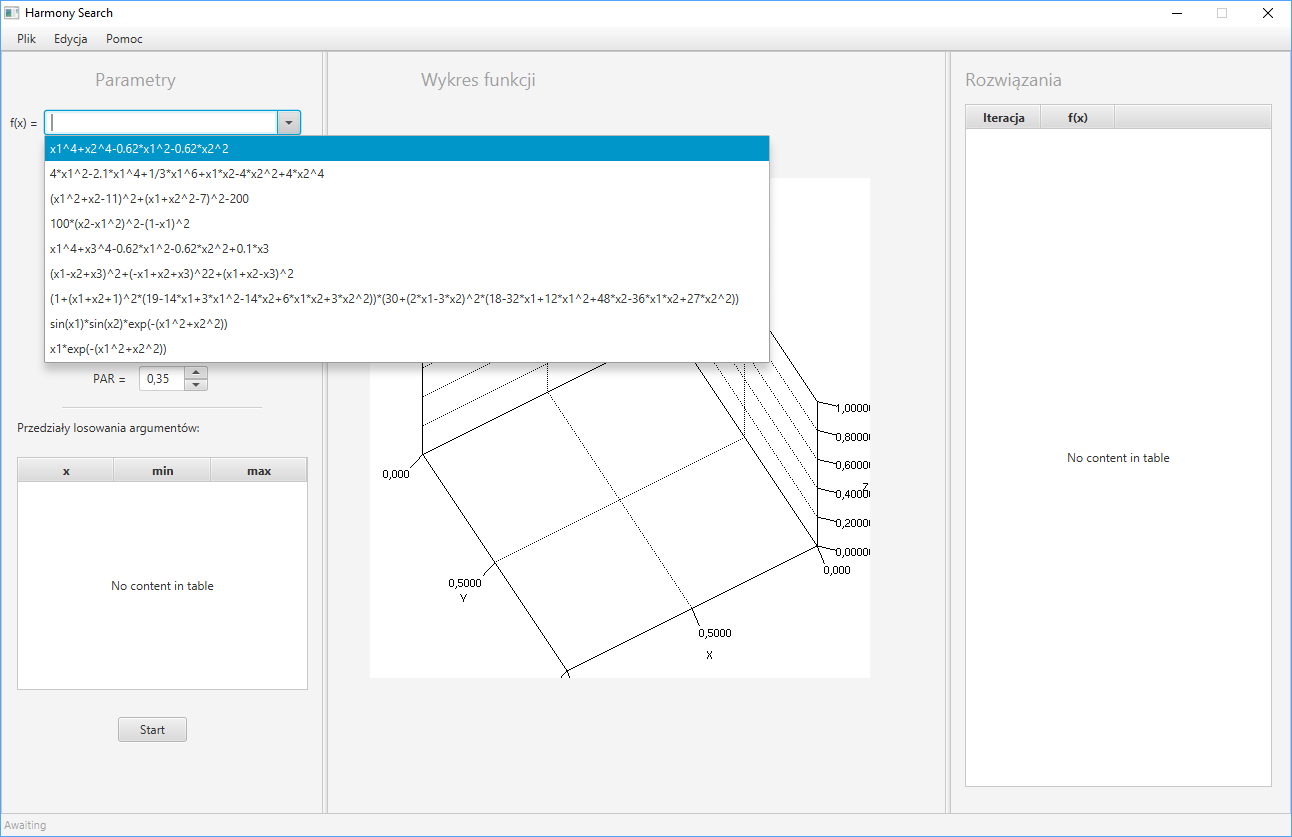
\includegraphics[width=.8\linewidth]{images/1.PNG} 
		\caption{Wpisywanie funkcji}
		\label{fig:1}
	\end{minipage} 
	\begin{minipage}[b]{.5\linewidth}
		\centering
		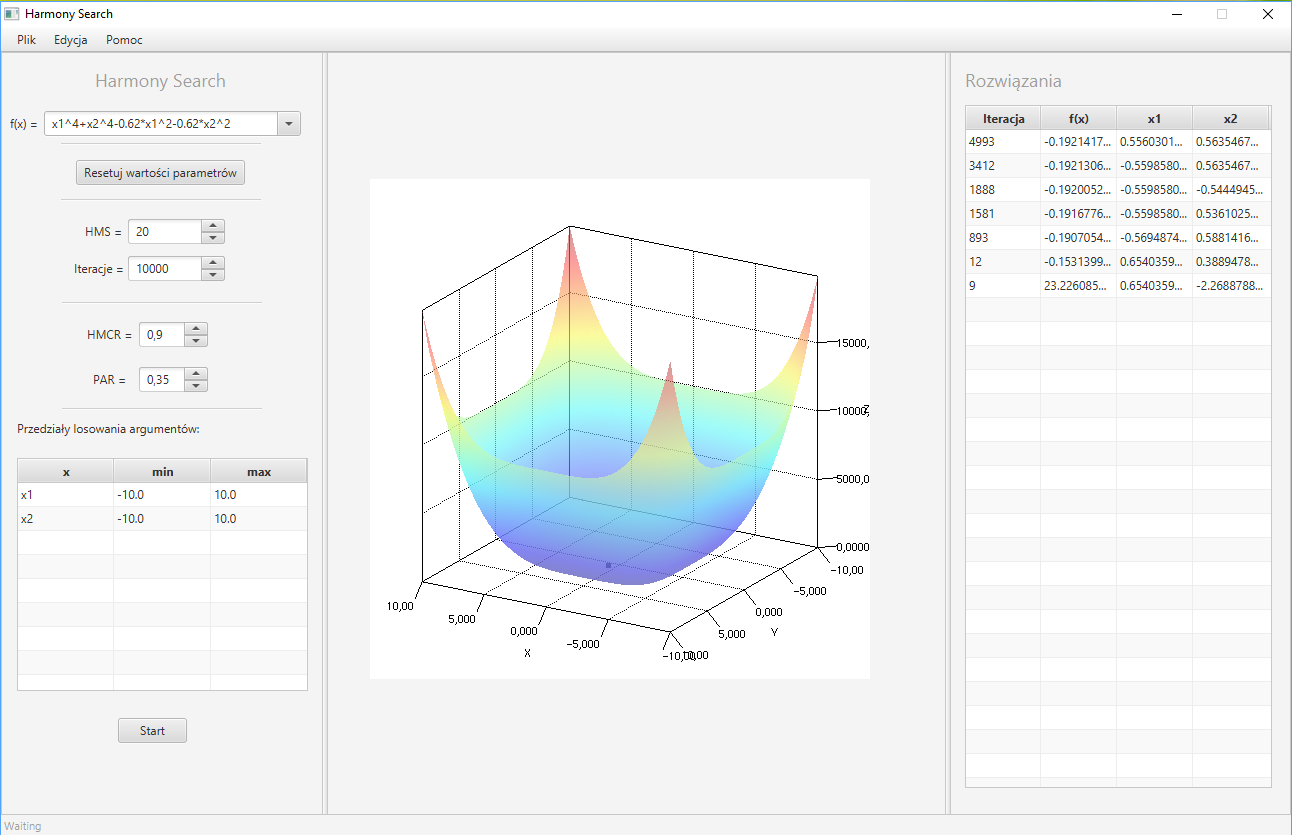
\includegraphics[width=.8\linewidth]{images/3.PNG} 
		\caption{Wykres z zaznaczonym rozwiązaniem}
		\label{fig:2}
	\end{minipage}
	\newline
	\newline
	\begin{minipage}[b]{1\linewidth}
		\centering
		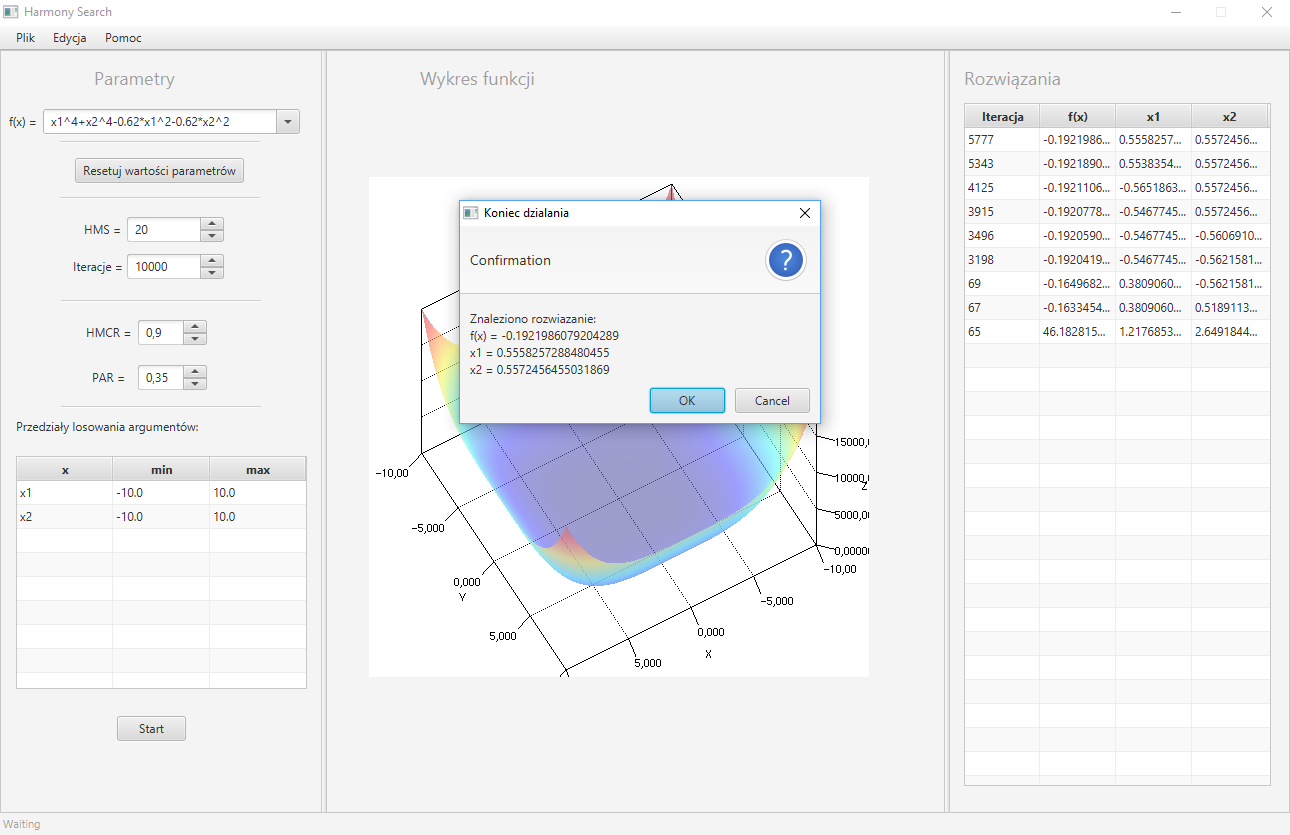
\includegraphics[width=.9\linewidth]{images/2.PNG} 
		\caption{Obliczone rozwiązanie wraz z komunikatem}
		\label{fig:3}
	\end{minipage}
\end{figure}

\subsubsection{Parametry}
\label{subsubsec:parametry}
W części parametrów można dostrzec, że zaraz pod paskiem edycji znajduje miejsce do wpisania funkcji. Jest to ta sama funkcja której minimum należy wyznaczyć. Okno umożliwia również wybór takiej funkcji z wcześniej zadeklarowanych w programie. Dokonuje się tego klikając w rozwijane menu. Zostało to przedstawione na rysunku \ref{fig:1}. Po wybraniu funkcji automatycznie zostaną domyślnie uzupełnione wszystkie parametry obliczeń. Oczywiście możliwa jest dostosowanie algorytmu do własnych potrzeb. Poniżej okna funkcji znajduje się przycisk ,,{\tt Resetuj wartości parametrów}'' umożliwiający, jak mówi nazwa, reset do parametrów domyślnych. Poniżej przycisku zostały umieszczone po sobie cztery główne parametry algorytmu {\em Harmony Search}. \\
Pierwszy z parametrów {\tt HMS} ({\em ang. harmony memory size}) reguluje ilość zapamiętywanych rozwiązań podczas wyszukiwania. Domyślnie rozmiar jest zadeklarowany na $20$. Poniżej znajduje się okno o nazwie {\tt iteracje}. Domyślnie jest zadeklarowana maksymalna wartość iteracji równa $10000$. W każdej iteracji programu algorytm wyszukuje nowe rozwiązanie i sprawdza je z tymi zapisanymi w {\tt HMS}. Czym większa ilość iteracji tym algorytm powinien obliczać dokładniejsze rozwiązanie, kosztem wydłużonego czasu obliczeń. Następnie pod polem {\tt iteracje} znajduje się pole {\tt HMCR} ({\em ang. harmony memory consideration ratio}). Tłumaczenie określa go jako współczynnik wyboru tonu z pamięci. Jest to współczynnik prawdopodobieństwa wybierany z zakresu $(0, 1)$. Czym {\tt HMCR} jest większe tym wyszukiwane wartości {\em x} następnych rozwiązań będą zbliżone do tych istniejących już w tablicy {\tt HMS}. Poniżej znajduje się drugi parametr prawdopodobieństwa dla funkcji o nazwie {\tt PAR} {\em(ang. pitch adjustment ratio)} tłumaczony jako współczynnik dostosowywania tonu. Wybierany jest również z zakresu $(0, 1)$. Na samym dole kolumny znajduje się tabela {\tt Przedziały losowania argumentów}. W tabeli deklarowany jest przedziały wszystkich wartości {\em x} dla których ma być poszukiwane rozwiązanie. Domyślnie parametry dla wszystkich {\em x} brane są z przedziału $(-10, 10)$. Algorytm z dużą dokładnością znajdzie najmniejsze minimum lokalne dla funkcji z podanego przedziału. Po wybraniu wszystkich parametrów można przystąpić do uruchomienia algorytmu przyciskiem {\tt Start} znajdującym się na na dole kolumny.

\subsubsection{Wykres}
\label{subsubsec:wykres}
Środkowy obszar okna głównego przeznaczony jest do wyświetlania wykresu funkcji. Jak wspomniane zostało na początku rozdziału \ref{sec:implementacja}, do rysowania wykresów została użyta zewnętrzna biblioteka {\em jzy3D}. Umożliwia ona tworzenie wykresów dwu i trzy wymiarowych.  Wykresy można obracać w dowolny sposób. Oś {\em X} i {\em Y} wykresu wyskalowana jest do najmniejszego i największego parametru wszystkich wartość {\em x}. Dodatkowo wartości zostały pokolorowane w tak, że mniejsze wartości funkcji mają kolory zimniejsze, a wyższe kolory cieplejsze, analogicznie do tego jak przedstawia się wysokość n.p.m. w kartografii. Dodatkowo czarną kropką zaznaczona została najmniejsza obliczona wartość funkcji. 

\subsubsection{Tabela Rozwiązań}
\label{subsubsec:rozwiazania}
Po prawej stronie okna głównego można dostrzec najlepsze rozwiązania wyszukane przez program. Gdy znajdowane jest rozwiązanie lepsze od najlepszego rozwiązania zapamiętanego w {\tt HMS} dodawane jest ono jako pierwszy wiersz w tabeli. Poprzednie rozwiązania przesuwane są o jedno miejsce niżej. Pozwala to śledzić jaka wartości jest aktualnie największa oraz od razu ukazuje się obok numer iteracji tego rozwiązania. Gdy algorytm długo oblicza najlepszy wynik okno pozwala śledzić postęp obliczeń. Dodatkowo po wykonaniu wszystkich iteracji zostaje wyświetlony komunikat z najlepszym rozwiązaniem (pierwszym od góry), co przedstawia rysunek \ref{fig:3}.

\subsection{Pliki}
\label{subsec:pliki}
Program był pisany w środowisku programistycznym {\em IntelliJ IDEA}. Jak wcześniej wspomniano do stworzenia GUI programu użyto technologii {\em JavaFx} umożliwiającej tworzenie aplikacji okienkowych. Dodatkowo by ułatwić zarządzanie bibliotekami wewnątrz programu użyto wsparcia ze strony {\em Maven}. Główny kod programu został umieszczony katalogu {\tt src}. Katalog zawiera w sobie dwa inne katalogi {\tt resourses} oraz {\tt java}. Katalog {\tt resourses} posiada jeden folder w którym umieszczony jest plik {\tt main.fxml} odpowiedzialny GUI programu. W tym pliku zapisane są informacje o ułożeniu i wielkości elementów, które widzi użytkownik. Można powiedzieć że plik odpowiada za foreground programu. \\
Cała background programu czyli jego mechanika jest umieszczona w folderze {\tt java}. Posiada on dwa podfoldery {\tt org.jzy3d} oraz {\tt com.blag.harmonysearch}. Pierwszy katalog odpowiedzialny jest za generowanie wykresów w oknie opisywanym w rozdziale \ref{subsubsec:wykres}. Są to pliki zewnętrzne pobrane ze strony \cite{bib:jzy3d}. Katalog {\tt com.blag.harmonysearch} zawiera cztery foldery. Każdy z nich posiada pliki napisane na potrzeby tego projektu. Dla czytelności opisu zostaną one przedstawione jako kolejne podrozdziały.

\newline \newline
\begin{forest}
	for tree={font=\sffamily, grow'=0, folder icons, edge=densely dotted}
	[/src/VIDEO/
	[ \ \ \ 17-11-26, this folder size=25pt
	[ \ \ CAM1, this folder size=18pt
	[17-11-27\_19.00.00.h264, is file]
	[17-11-27\_19.00.00.h264, is file]]]
	[ \ \ \ 17-11-25, this folder size=25pt]
	[ \ \ \ 17-11-25, this folder size=25pt]
	]
\end{forest}
\newline

\subsubsection{Katalog contants}
\ref{subsubsec:contants}

\subsubsection{Katalog core}
\ref{subsubsec:core}

\subsubsection{Katalog gui}
\ref{subsubsec:gui}

\subsubsection{Katalog helpers}
\ref{subsubsec:helpers}

\section{Przykładowe rozwiązania}
\label{sec:przyklady}
W tej części zostały przedstawione trzy przykłady funkcji dwóch zmiennych {\em $x_{1}$} i {\em $x_{2}$} wraz z obliczonymi rozwiązaniami. 

\subsection{Funkcja czterech minimum}
\label{subsec:fcn4min}
Pierwsza zostanie przedstawiona funkcja posiadająca cztery minima lokalne. Posiada ona następujący wzór: $$f(x) = x_{1}^{4}+x_{2}^{4}-0.62x_{1}^{2}-0.62x_{2}^{2} $$ Na przykładzie tej funkcji zostało również omówione GUI programu w rozdziale \ref{subsec:gui}. Rysunek \ref{fig:4} prezentuje wykres funkcji wraz z najlepszą wartością. Dokładną wartość można odczytać po prawej stronie i jest to 4993 iteracja równa $f(0.5560,0.5635) = -0.1914$. Poniżej zaprezentowany jest wykres funkcji. 
\begin{figure}[htbp]
	\centering
		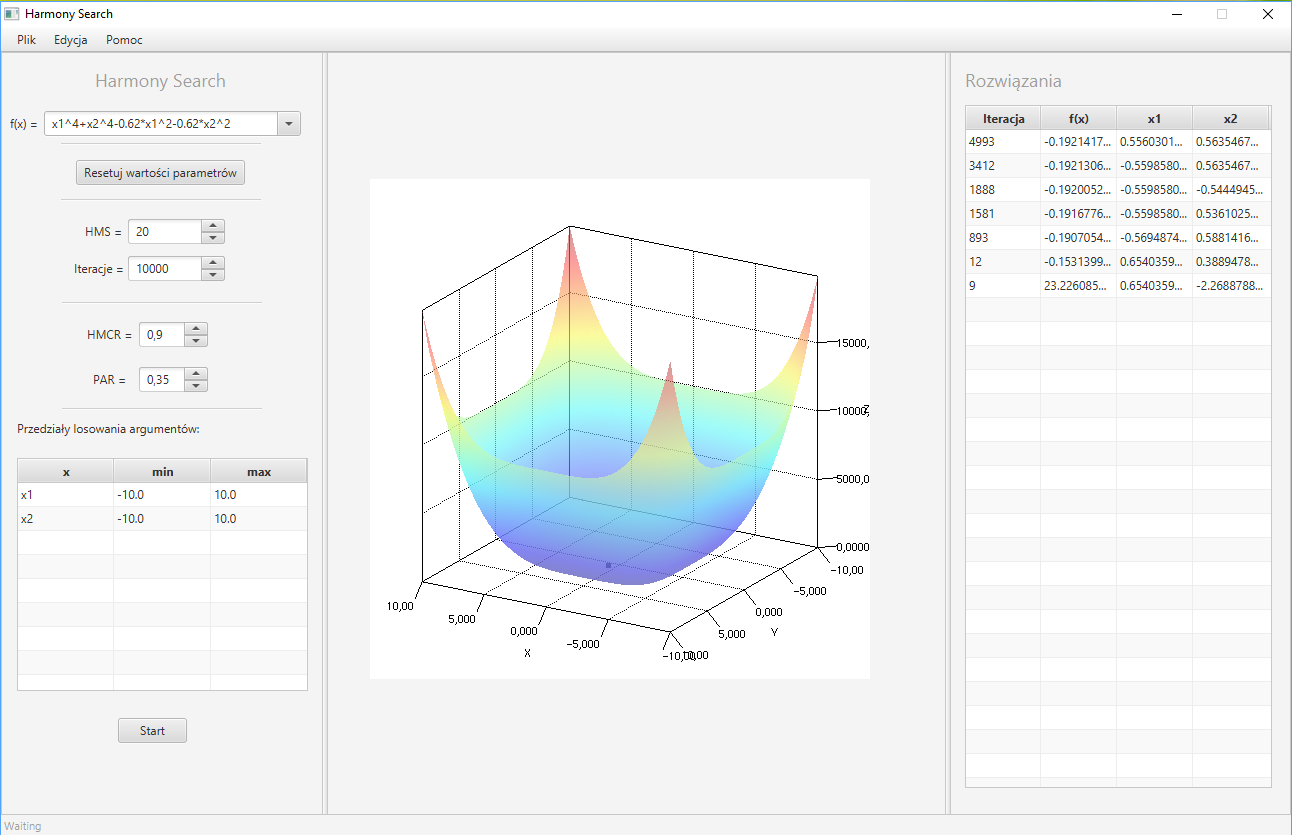
\includegraphics[width=0.90\textwidth]{images/3.PNG}
		\caption{Wykres funkcji czterech minimum}
		\label{fig:4}
\end{figure}

\subsection{Funkcja Himmelblau}
\label{subsec:himmelblau}
Funkcja Himmelbalu również jak \ref{subsec:fcn4min} posiada cztery minima lokalne zlokalizowane po jednym w każdej ćwiartce na przedziale $x_{1,2} \in (-5,5)$. Funkcja posiada wzór: $$ f)x) = (x_{1}^{2}+x_{2}-11)^{2}+(x_{1}+x_{2}^{2}-7)^{2}-200$$. Dla pokazania, że funkcja wyszukuje rozwiązania z innego przedziału jak domyślny ograniczono się do przedziału z pierwszej ćwiartki $x_{1}, x_{2} \in (0,10)$. Na wykresie \ref{fig:5} zaprezentowany został wykres funkcji wraz z naniesionym najlepszym rozwiązaniem. 
\begin{figure}[htbp]
	\centering
	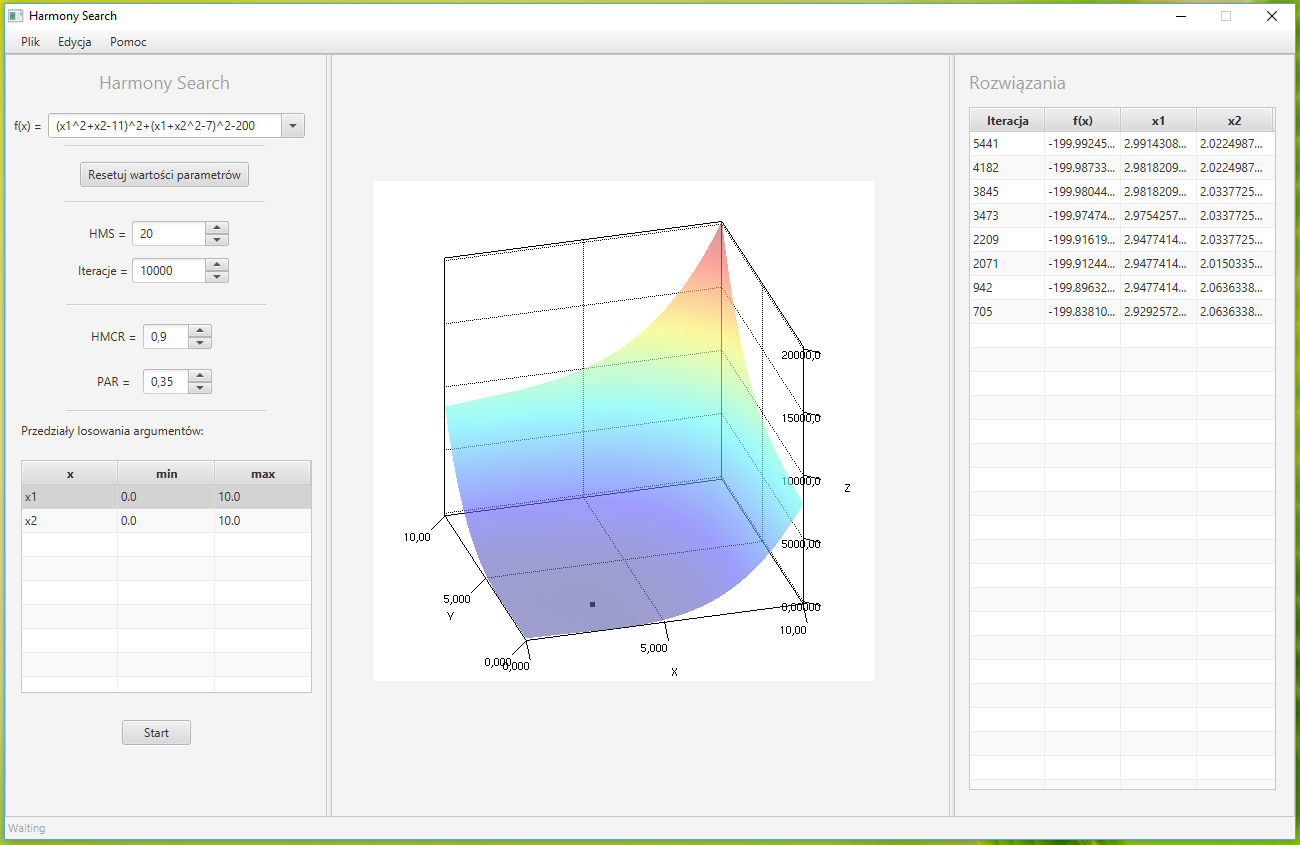
\includegraphics[width=0.90\textwidth]{images/4.PNG}
	\caption{Wykres funkcji Himmelblau}
	\label{fig:5}
\end{figure}

\subsection{Funkcja sinus-cosinus z eksponentom}
\label{subsec:sinexp}
Ostatnia przedstawiana funkcja ukazuje przypadek połączenia funkcji sinusa-cosinusa z eksponent. Przypadek jest o tyle ciekawy, że większość wartości funkcji jest dla {\em $x_{1}, x_{2}$} jest do siebie zbliżona. Blisko jej wartość ulega dużemu odchyłowi.  Wzór funkcji przedstawiony jest jako: $$x_{1}e^{-(x_{1}^{2}+x_{2}^2)}$$. Rysunek \ref{fig:6} prezentuje działanie programu z obliczoną wartością minimalną. Jak możemy dostrzec program dobrze wyliczył jej wartość co potwierdza jego odporność na działanie funkcji, dla której większość argumentów jest stała. 
\begin{figure}[htbp]
	\centering
	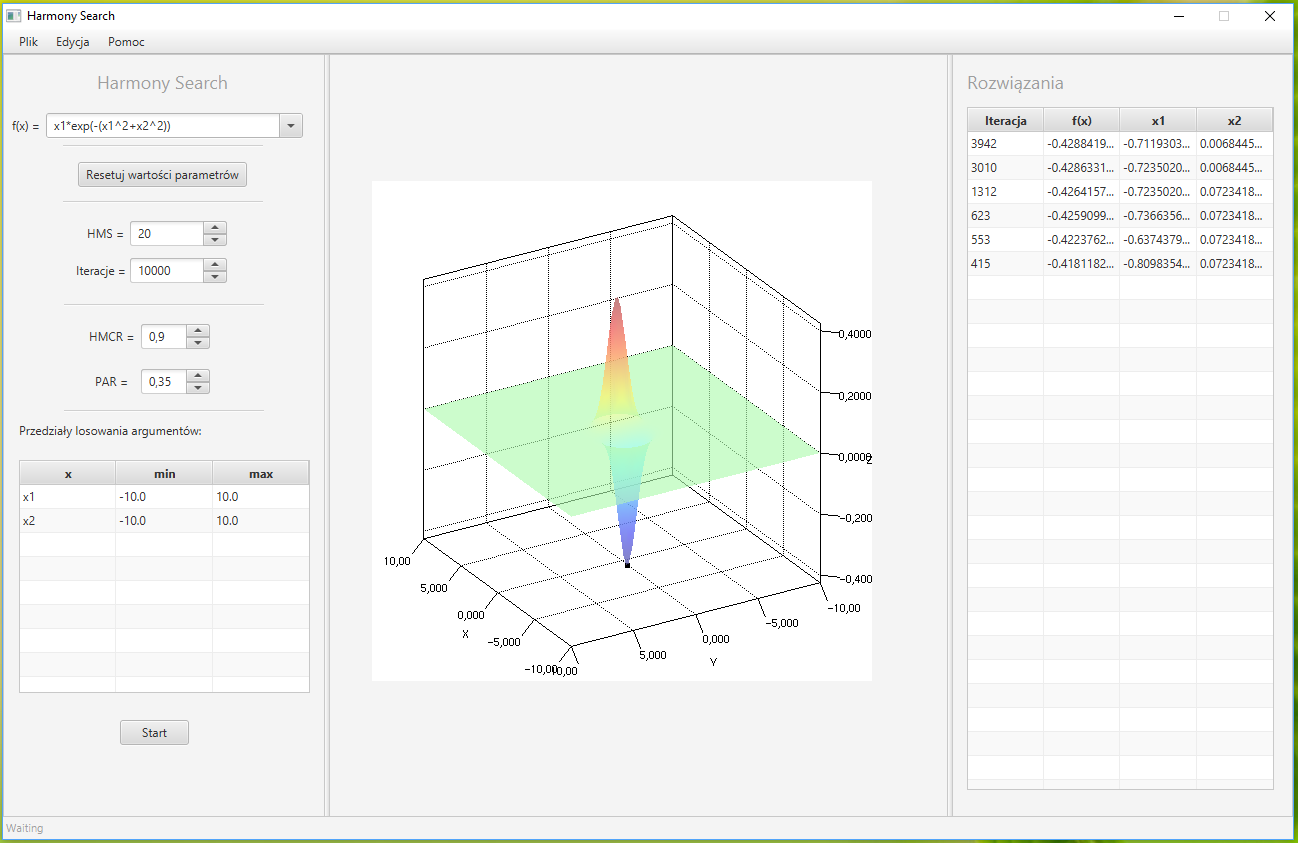
\includegraphics[width=0.90\textwidth]{images/5.PNG}
	\caption{Wykres funkcji sinusa-cosinusa z eksponentom}
	\label{fig:6}
\end{figure}

\section{Problemy podczas pracy}
\label{sec:problemy}
Jednym z problemów z jakim musiał poradzić sobie program było prezentowanie danych. Algorytm jest zdolny do obliczania funkcji wielu zmiennych dla {\em $x_{n} , n \in N$}. Prezentowanie zmiennych w tabelach jest rzeczą dającą się w prosty sposób rozwinąć. Jednak rysowanie wykresu dla $n \leq 2$ ilości zmiennych nie jest możliwy. Najładniejsze wykresy powstają dla $n = 2$ dlatego funkcje o dwóch zmiennych zostały przedstawione w rozdziale \ref{sec:przyklady}. \\

\section{Podsumowanie}
\label{sec:podsumowanie}


\newpage
\addcontentsline{toc}{section}{Bibilografia}
\bibliography{bibliografia}
\bibliographystyle{plain}

\end{document}

